\documentclass{tufte-handout}

\usepackage{amsmath}
\usepackage{graphicx}
\setkeys{Gin}{width=\linewidth,totalheight=\textheight,keepaspectratio}
\graphicspath{{images/}}
\usepackage{booktabs}
\usepackage{units}
\usepackage{fancyvrb}
\fvset{fontsize=\normalsize}

\title{Measuring the speed of light}
\author[John P. Cummings]{John P. Cummings}
% \date{24 January 2009}  % if the \date{} command is left out, the current date will be used


\begin{document}

\maketitle% this prints the handout title, author, and date

\begin{abstract}
\noindent In this lab you'll see how Ole R{\o}mer used variations in the observed times of Io solar eclipses by Jupiter to determine the speed of light in 1676.  You will use data from recent observations to reproduce R{\o}mers measurement and determine the value of $c$ yourself.
\end{abstract}


\section{History}
\newthought{Attempts to measure} the speed of light go back hundreds of years.  Galileo Galelei describes an attempt to measure the speed of light in 1638.  In Dialogues Concerning Two New Sciences\footnote{\url{http://oll.libertyfund.org/?option=com_staticxt&staticfile=show.php\%3Ftitle=753}}, Salviati describes to Sagredo and Simplicio an experiment that we assume was performed by Galileo:  two men, equipped with shuttered lanterns, climb to the tops of hills about one mile apart.  The first man opens the shutter of his lantern and the second man, as soon as he sees the light from the first, opens the shutter on his lantern.  The first man then notes the time that passes between his opening the shutter and seeing the light from the second lantern.   With this time and the distance between lanterns, he can then calculate the speed of light.  
\begin{figure}
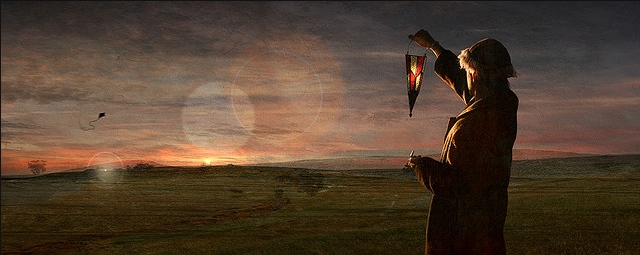
\includegraphics{galileo_beacon_of_gondor.jpg}
\end{figure}

Galileo's report of his conclusion is interesting.  He realizes that the error inherent in his experiment, dominated by the reaction time of the lantern operators, limits the maximum speed he can measure, and thus he can only set a lower bound:

\begin{quote}
In fact I have tried the experiment only at a short distance, less than a mile, from which I have not been able to ascertain with certainty whether the appearance of the opposite light was instantaneous or not; but if not instantaneous it is extraordinarily rapid.
\end{quote}

%1676 - romer reports to french academy
\newthought{The first finite measurement} was made (as often happens in science) by accident.  in the late 1600's, Ole R{\o}mer was studying the eclipses of one of Jupiters largest moons, Io.
\begin{marginfigure}
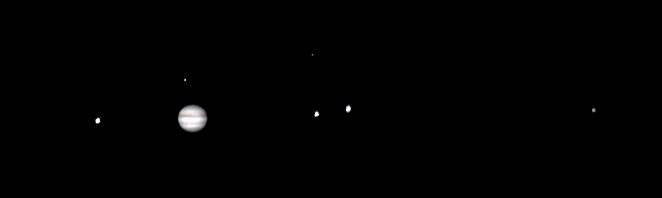
\includegraphics{Romer2.jpg}
\caption{Jupiter and its Galilean moons}
\end{marginfigure}
At the time, it was difficult for navigators to determine their longitude, since this required an accurate clock, which did not exist at the time.  Galileo had suggested that the timing of Io's eclipses could be used as a celestial clock, and in fact this method was the best until improvements in mechanical clocks surpassed it in the 1800's.  R{\o}mer was making careful measurements of the times of Io's eclipses for this purpose when he noticed that there were irregularities in the times.  He noticed that the period between eclipses was slightly longer when the earth was moving away from Jupiter, and slightly shorter when moving towards it.
 His great insight was that this was due to the finte speed of light.  He presented this argument to the French Academy of Sciences in 1676.

\section{R{\o}mer's measurement}

To aid the discussion of R{\o}mer's measurement, let's familiarize ourselves with some astronomical terms and concepts.
\begin{description}
\item[conjunction] occurs when Jupiter and the Sun have the same right ascension, as viewed from earth.  Basically Jupiter and the Sun pass each other in the sky.
\item[opposition] occurs when Jupiter and the Sun are at their largest angular separation in the sky, as viewed from earth: Jupiter and the Sun are opposite each other in the sky. 
\end{description}

Examine Figure~\ref{fig:JupIo}. The Earth is between a conjunction and an opposition. The radius of the orbit of Io is equal to six times the radius of Jupiter. The angle $SJT = \theta$ is always smaller than 11 deg.
\begin{figure}
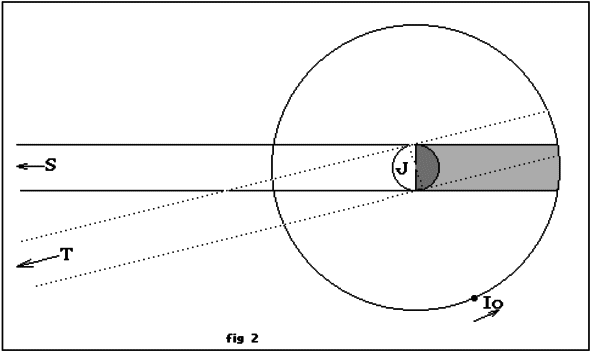
\includegraphics{RomerFig2.png}
\caption{Jupiter (J) , Io (Io) and the directions of the Sun (S) and the Earth (T) at a point between a conjunction and an opposition.}
\label{fig:JupIo}
\end{figure}
On this figure, indicate the points where the beginning and the end of the following four phenomena take place:
\begin{description}[itemsep=0pt,parsep=0pt,topsep=0pt,partopsep=0pt]
\item[Eclipse] The satellite enters the shadow of Jupiter.
\item[Occultation] The satellite, as seen from Earth, goes behind Jupiter.
\item[Shadow] The shadow of the satellite is seen on the planet.
\item[Passage] The satellite, as seen from Earth, passes in front of the planet.
\end{description}

\begin{itemize}
\item Now explain why only the beginnings of the eclipses can be observed from Earth.
\item What happens when the Earth is close to a conjunction?
\item Draw another figure that shows what happens when the Earth is between an opposition and a conjunction. 
\item Explain why then only the ends of the eclipses can be observed from Earth.
\end{itemize}

We can now look at how R{\o}mer measured the speed of light.
\begin{marginfigure}
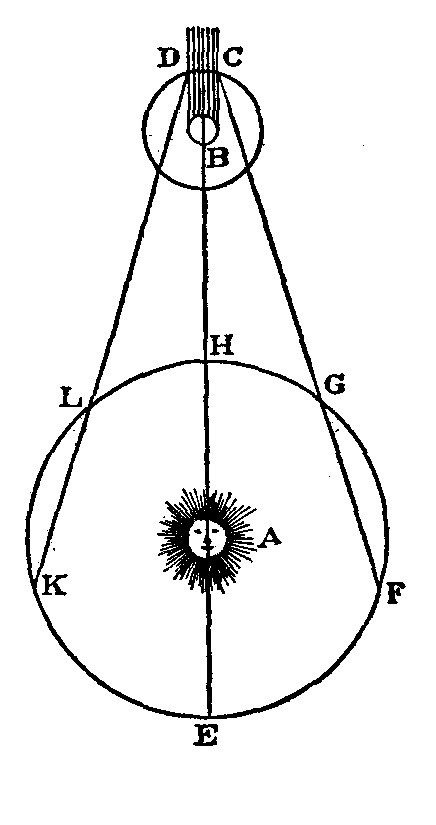
\includegraphics{Roemer.jpg}
\caption{From the 1676 article describing R{\o}mer's method. Both Earth and Io are moving counterclockwise in this image.}
\label{fig:sunJup}
\end{marginfigure}
Looking at figure~\ref{fig:sunJup} he noticed that if he used the times of the eclipses at point $L$ or $H$ as a ``start time" to then predict the times of subsequent ellipses, then the end of eclipses at $K$ or $E$ seemed to happen later than he would expect. He reasoned that this delay was caused by the extra time it took light to propagate this extra distance. 

Although R{\o}mer never calculated a value for the speed of light, Christian Huygens quickly got R{\o}mer's data and did so, getting a value of $16 \frac{2}{3}$ Earth diameters per second (or $2.125\times10^8~{\rm m}/{\rm s}$).  Pretty good for 1676!

\section{A modern recalculation}

The exercise for this lab is to reconstruct R{\o}mers argumant and recalculate using modern observations.  Below is a table of eclipse timings from the mid 1990's.  This table, which I will also provide as a text file also so you can read it into the programming/calculation tool of your choice, and the radius of the Earth's orbit is all you should need to calculate $c$.

You should first use the data to determine the period of Io.  I would suggest using data from a region of Earth's orbit that is not affected significantly by the finite speed of light.  What part of the Earth's orbit meets this criterion? {\it Check with the instructor that your period is reasonable, before proceeding with the rest of the lab.}

Once you have determined a period, use it to predict the time of a later eclipse (either beginning or end of eclipse, depending on the data you are using).  Once you have the predicted time, find the difference in time with the corresponding eclipse observation from the tables.  By using this time difference and the distance the earth has moved between the two eclipse observations, you should be able to calculate the speed of light.

If you are reading the data files using a programming language like python, I would suggest spending a few minutes building some tools to help your analysis. 
For example, you may want to write functions that
\begin{itemize}
    \item Takes in a filename and reads the data into an array or arrays.
    \item Takes the date and time format given in the data files and returns a format you can work with, either seconds or, if you are using python, using the {\tt datetime} library.
\end{itemize}

If you have these functions, performing the rest of the calculation should be straightforward. For those of you using a tool that allows you to 
plot your data, you are encouraged to come up with plots or visualizations of your approach.

If you are not comfortable with a programming language like python, you can get quite far using a spreadsheet like Excel or Google Sheets.

\newthought{Those of you} doing the exercise ``by hand'' might find Wolfram Alpha useful for such things as finding the difference between two dates.  Visit the Alpha website and experiment with various date formats to make sure you understand the answers it gives you.


\begin{table*}
\begin{tabular}{lll|lll|lll}
\# & date & time & \# & date & time & \# & date & time \\ \hline
00 & 14/12/94 & 08h37 & 34 & 12/02/95 & 12h41 & 68 & 13/04/95 & 16h41 \\
01 & 16/12/94 & 03h06 & 35 & 14/02/95 & 07h09 & 69 & 15/04/95 & 11h09 \\
02 & 17/12/94 & 21h34 & 36 & 16/02/95 & 01h37 & 70 & 17/04/95 & 05h37 \\
03 & 19/12/94 & 16h03 & 37 & 17/02/95 & 20h05 & 71 & 19/04/95 & 00h05 \\
04 & 21/12/94 & 10h31 & 38 & 19/02/95 & 14h34 & 72 & 20/04/95 & 18h34 \\
05 & 23/12/94 & 04h59 & 39 & 21/02/95 & 09h02 & 73 & 22/04/95 & 13h02 \\
06 & 24/12/94 & 23h28 & 40 & 23/02/95 & 03h30 & 74 & 24/04/95 & 07h30 \\
07 & 26/12/94 & 17h56 & 41 & 24/02/95 & 21h58 & 75 & 26/04/95 & 01h59 \\
08 & 28/12/94 & 12h25 & 42 & 26/02/95 & 16h27 & 76 & 27/04/95 & 20h27 \\
09 & 30/12/94 & 06h53 & 43 & 28/02/95 & 10h55 & 77 & 29/04/95 & 14h55 \\
10 & 01/01/95 & 01h21 & 44 & 02/03/95 & 05h23 & 78 & 01/05/95 & 09h23 \\
11 & 02/01/95 & 19h50 & 45 & 03/03/95 & 23h51 & 79 & 03/05/95 & 03h52 \\
12 & 04/01/95 & 14h18 & 46 & 05/03/95 & 18h19 & 80 & 04/05/95 & 22h20 \\
13 & 06/01/95 & 08h46 & 47 & 07/03/95 & 12h48 & 81 & 06/05/95 & 16h48 \\
14 & 08/01/95 & 03h15 & 48 & 09/03/95 & 07h16 & 82 & 08/05/95 & 11h17 \\
15 & 09/01/95 & 21h43 & 49 & 11/03/95 & 01h44 & 83 & 10/05/95 & 05h45 \\
16 & 11/01/95 & 16h11 & 50 & 12/03/95 & 20h12 & 84 & 12/05/95 & 00h14 \\
17 & 13/01/95 & 10h40 & 51 & 14/03/95 & 14h41 & 85 & 13/05/95 & 18h42 \\
18 & 15/01/95 & 05h08 & 52 & 16/03/95 & 09h09 & 86 & 15/05/95 & 13h10 \\
19 & 16/01/95 & 23h36 & 53 & 18/03/95 & 03h37 & 87 & 17/05/95 & 07h39 \\
20 & 18/01/96 & 18h05 & 54 & 19/03/95 & 22h05 & 88 & 19/05/95 & 02h07 \\
21 & 20/01/95 & 12h33 & 55 & 21/03/95 & 16h33 & 89 & 19/05/95 & 20h36 \\
22 & 22/01/95 & 07h01 & 56 & 23/03/95 & 11h02 & 90 & 22/05/95 & 15h04 \\
23 & 24/01/95 & 01h30 & 57 & 25/03/95 & 05h30 & 91 & 24/05/95 & 09h32 \\
24 & 25/01/95 & 19h56 & 58 & 26/03/95 & 23h58 & 92 & 26/05/95 & 04h01 \\
25 & 27/01/95 & 14h26 & 59 & 28/03/95 & 18h26 & 93 & 27/05/95 & 22h29 \\
26 & 29/01/95 & 08h55 & 60 & 30/03/95 & 12h55 & 94 & 29/05/95 & 16h58 \\
27 & 31/01/95 & 03h23 & 61 & 01/04/95 & 07h23 & 95 & 31/05/95 & 11h26 \\
28 & 01/02/95 & 21h51 & 62 & 03/04/95 & 01h51 &  & & \\
29 & 03/02/95 & 16h19 & 63 & 04/04/95 & 20h19 &  & & \\
30 & 05/02/95 & 10h48 & 64 & 06/04/95 & 14h48 &  & & \\
31 & 07/02/95 & 05h16 & 65 & 08/04/95 & 09h16 &  & & \\
32 & 08/02/95 & 23h44 & 66 & 10/04/95 & 03h44 &  & & \\
33 & 10/02/95 & 18h12 & 67 & 11/04/95 & 22h12 &  & & \\
\end{tabular}
\caption{ Begin of Eclipse between the conjunction on November 17, 1994 (20h00) and the opposition on June 1, 1995 (11h00). }
\end{table*}

\begin{table*}
\begin{tabular}{lll|lll|lll}
\# & date & time & \# & date & time & \# & date & time \\ \hline\\
00 & 02/06/95 & 08h06 & 34 & 01/08/95 & 12h20 & 68 & 30/09/95 & 16h40\\
01 & 04/06/95 & 02h34 & 35 & 03/08/95 & 06h48 & 69 & 02/10/95 & 11h09\\
02 & 05/06/95 & 21h03 & 36 & 05/08/95 & 01h17 & 70 & 04/10/95 & 05h37\\
03 & 07/06/95 & 15h31 & 37 & 06/08/95 & 09h56 & 71 & 06/10/95 & 00h06\\
04 & 09/06/95 & 10h00 & 38 & 08/08/95 & 14h15 & 72 & 07/10/95 & 18h35\\
05 & 11/06/95 & 04h28 & 39 & 10/08/95 & 08h44 & 73 & 09/10/95 & 13h04\\
06 & 12/06/95 & 22h57 & 40 & 12/08/95 & 03h12 & 74 & 11/10/95 & 07h33\\
07 & 14/06/95 & 17h25 & 41 & 13/08/95 & 21h41 & 75 & 13/10/95 & 02h01\\
08 & 16/06/95 & 11h54 & 42 & 15/08/95 & 16h10 & 76 & 14/10/95 & 20h30\\
09 & 18/06/95 & 06h22 & 43 & 17/08/95 & 10h39 & 77 & 16/10/95 & 14h59\\
10 & 20/06/95 & 00h51 & 44 & 19/08/95 & 05h08 & 78 & 18/10/95 & 09h28\\
11 & 21/06/95 & 19h20 & 45 & 20/08/95 & 23h26 & 79 & 20/10/95 & 03h57\\
12 & 23/06/95 & 13h48 & 46 & 22/08/95 & 18h05 & 80 & 21/10/95 & 22h26\\
13 & 25/06/95 & 08h17 & 47 & 24/08/95 & 12h34 & 81 & 23/10/95 & 16h54\\
14 & 27/06/95 & 02h45 & 48 & 26/08/95 & 07h03 & 82 & 25/10/95 & 11h23\\
15 & 28/06/95 & 21h14 & 49 & 28/08/95 & 01h32 & 83 & 27/10/95 & 05h52\\
16 & 30/06/95 & 15h43 & 50 & 29/08/95 & 20h00 & 84 & 29/10/95 & 00h21\\
17 & 02/07/95 & 10h11 & 51 & 31/08/95 & 14h29 & 85 & 30/10/95 & 18h50\\
18 & 04/07/95 & 04h40 & 52 & 02/09/95 & 08h58 & 86 & 01/11/95 & 13h18\\
19 & 05/07/95 & 23h09 & 53 & 04/09/95 & 03h27 & 87 & 03/11/95 & 07h47\\
20 & 07/07/95 & 17h37 & 54 & 05/09/95 & 21h56 & 88 & 05/11/95 & 02h16\\
21 & 09/07/95 & 12h06 & 55 & 07/09/95 & 16h25 & 89 & 06/11/95 & 20h45\\
22 & 11/07/95 & 06h35 & 56 & 09/09/95 & 10h54 & 90 & 08/11/95 & 15h13\\
23 & 13/07/95 & 01h03 & 57 & 11/09/95 & 05h22 & 91 & 10/11/95 & 09h42\\
24 & 14/07/95 & 19h32 & 58 & 12/09/95 & 23h51 & 92 & 12/11/95 & 04h11\\
25 & 16/07/95 & 14h01 & 59 & 14/09/95 & 18h20 & 93 & 13/11/95 & 22h40\\
26 & 18/07/95 & 08h30 & 60 & 16/09/95 & 12h49 & 94 & 15/11/95 & 17h09\\
27 & 20/07/95 & 02h58 & 61 & 18/09/95 & 07h18 & 95 & 17/11/95 & 11h37\\
28 & 21/07/95 & 21h27 & 62 & 20/09/95 & 01h47 & 96 & 19/11/95 & 06h06\\
29 & 23/07/95 & 15h56 & 63 & 21/09/95 & 20h15 & 97 & 21/11/95 & 00h35\\
30 & 25/07/95 & 10h24 & 64 & 23/09/95 & 14h44 & 98 & 22/11/95 & 19h04\\
31 & 27/07/95 & 04h53 & 65 & 25/09/95 & 09h13 & & &\\
32 & 28/07/95 & 23h22 & 66 & 27/09/95 & 03h42 & & &\\
33 & 30/07/95 & 17h51 & 67 & 28/09/95 & 22h11 & & &\\
\end{tabular}
\caption{End of Eclipse between the opposition on June 1, 1995 (11:00) and the conjunction on December 18, 1995 (22:00)}
\end{table*}


\begin{table*}
\begin{tabular}{lll|lll|lll}
\# & date & time & \# & date & time & \# & date & time \\ \hline
00 & 14/01/96 & 19h09 & 34 & 14/03/96 & 23h15 & 68 & 14/05/96 & 03h18\\
01 & 16/01/96 & 13h38 & 35 & 16/03/96 & 17h44 & 69 & 15/05/96 & 21h46\\
02 & 18/01/96 & 08h06 & 36 & 18/03/96 & 12h12 & 70 & 17/05/96 & 16h15\\
03 & 20/01/96 & 02h35 & 37 & 20/03/96 & 06h40 & 71 & 19/05/96 & 10h43\\
04 & 21/01/96 & 21h03 & 38 & 22/03/96 & 01h29 & 72 & 21/05/96 & 05h11\\
05 & 23/01/96 & 21h03 & 39 & 23/03/96 & 19h37 & 73 & 22/05/96 & 23h40\\
06 & 25/01/96 & 10h00 & 40 & 25/03/96 & 14h05 & 74 & 24/05/96 & 18h08\\
07 & 27/01/96 & 04h29 & 41 & 27/03/96 & 08h34 & 75 & 26/05/96 & 12h36\\
08 & 28/01/96 & 22h57 & 42 & 29/03/96 & 03h02 & 76 & 28/05/96 & 07h05\\
09 & 30/01/96 & 17h25 & 43 & 30/03/96 & 21h30 & 77 & 30/05/96 & 01h33\\
10 & 01/02/96 & 11h54 & 44 & 01/04/96 & 15h59 & 78 & 31/05/96 & 20h01\\
11 & 03/02/96 & 06h22 & 45 & 03/04/96 & 10h27 & 79 & 02/06/96 & 14h30\\
12 & 05/02/96 & 00h51 & 46 & 05/04/96 & 04h55 & 80 & 04/06/96 & 08h58\\
13 & 06/02/96 & 19h19 & 47 & 06/04/96 & 23h24 & 81 & 06/06/96 & 03h26\\
14 & 08/02/96 & 13h48 & 48 & 08/04/96 & 17h52 & 82 & 07/06/96 & 21h55\\
15 & 10/02/96 & 08h16 & 49 & 10/04/96 & 12h20 & 83 & 09/06/96 & 16h23\\
16 & 12/02/96 & 02h45 & 50 & 12/04/96 & 06h48 & 84 & 11/06/96 & 10h52\\
17 & 13/02/96 & 21h13 & 51 & 14/04/96 & 01h17 & 85 & 13/06/96 & 05h20\\
18 & 15/02/96 & 15h41 & 52 & 15/04/96 & 19h45 & 86 & 17/06/96 & 23h48\\
19 & 17/02/96 & 10h10 & 53 & 17/04/96 & 14h13 & 87 & 16/06/96 & 18h17\\
20 & 19/02/96 & 04h38 & 54 & 19/04/96 & 08h42 & 88 & 18/06/96 & 12h45\\
21 & 20/02/96 & 23h07 & 55 & 21/04/96 & 03h10 & 89 & 20/06/96 & 07h14\\
22 & 22/02/96 & 17h35 & 56 & 22/04/96 & 21h38 & 90 & 22/06/96 & 01h42\\
23 & 24/02/96 & 12h03 & 57 & 24/04/96 & 16h07 & 91 & 23/06/96 & 20h11\\
24 & 26/02/96 & 06h32 & 58 & 26/04/96 & 10h35 & 92 & 25/06/96 & 14h39\\
25 & 28/02/96 & 01h00 & 59 & 28/04/96 & 05h03 & 93 & 27/06/96 & 09h08\\
26 & 29/02/96 & 19h29 & 60 & 29/04/96 & 23h31 & 94 & 29/06/96 & 03h36\\
27 & 02/03/96 & 13h57 & 61 & 01/05/96 & 18h00 & 95 & 30/06/96 & 22h04\\
28 & 04/03/96 & 08h25 & 62 & 03/05/96 & 12h28 & 96 & 02/07/96 & 16h33\\
29 & 06/03/96 & 02h54 & 63 & 05/05/96 & 06h56 & & &\\
30 & 07/03/96 & 21h22 & 64 & 07/05/96 & 01h25 & & &\\
31 & 09/03/96 & 15h50 & 65 & 08/05/96 & 19h53 & & & \\
32 & 11/03/96 & 10h19 & 66 & 10/05/96 & 14h21 & & &\\
33 & 13/03/96 & 04h47 & 67 & 12/05/96 & 08h50 & & &\\
\end{tabular}
\caption{Begin of Eclipse between the conjunction on December 18, 1995 (22h00) and the opposition on July 4, 1996 (12h00).}
\end{table*}

\begin{table*}
\begin{tabular}{lll|lll|lll}
\# & date & time & \# & date & time & \# & date & time \\ \hline
00 & 04/07/96 & 13h16 & 34 & 02/09/96 & 17h31 & 68 & 01/11/96 & 21h51\\
01 & 06/07/96 & 07h45 & 35 & 04/09/96 & 12h00 & 69 & 03/11/96 & 16h20\\
02 & 08/07/96 & 02h13 & 36 & 06/09/96 & 06h28 & 70 & 05/11/96 & 10h49\\
03 & 09/07/96 & 20h42 & 37 & 08/09/96 & 00h57 & 71 & 07/11/96 & 05h18\\
04 & 11/07/96 & 15h10 & 38 & 09/09/96 & 19h26 & 72 & 08/11/96 & 23h47\\
05 & 13/07/96 & 09h39 & 39 & 11/09/96 & 13h55 & 73 & 10/11/96 & 18h16\\
06 & 15/07/96 & 04h08 & 40 & 13/09/96 & 08h24 & 74 & 12/11/96 & 12h44\\
07 & 16/07/96 & 22h36 & 41 & 15/09/96 & 02h52 & 75 & 14/11/96 & 07h13\\
08 & 18/07/96 & 17h05 & 42 & 16/09/96 & 21h21 & 76 & 16/11/96 & 01h42\\
09 & 20/07/96 & 11h33 & 43 & 18/09/96 & 15h50 & 77 & 17/11/96 & 20h11\\
10 & 22/07/96 & 06h02 & 44 & 20/09/96 & 10h19 & 78 & 19/11/96 & 14h40\\
11 & 24/07/96 & 00h31 & 45 & 22/09/96 & 04h48 & 79 & 21/11/96 & 09h09\\
12 & 25/07/96 & 18h59 & 46 & 23/09/96 & 23h17 & 80 & 23/11/96 & 03h37\\
13 & 27/07/96 & 13h28 & 47 & 25/09/96 & 17h45 & 81 & 24/11/96 & 22h06\\
14 & 29/07/96 & 07h56 & 48 & 27/09/96 & 12h14 & 82 & 26/11/96 & 16h35\\
15 & 31/07/96 & 02h25 & 49 & 29/09/96 & 06h43 & 83 & 28/11/96 & 11h04\\
16 & 01/08/96 & 20h54 & 50 & 01/10/96 & 01h12 & 84 & 30/11/96 & 05h33\\
17 & 03/08/96 & 15h22 & 51 & 02/10/96 & 19h41 & 85 & 02/12/96 & 00h02\\
18 & 05/08/96 & 09h51 & 52 & 04/10/96 & 14h10 & 86 & 03/12/96 & 18h31\\
19 & 07/08/96 & 04h20 & 53 & 06/10/96 & 08h38 & & &\\
20 & 08/08/96 & 22h48 & 54 & 08/10/96 & 03h07 & & &\\
21 & 10/08/96 & 17h17 & 55 & 09/10/96 & 21h36 & & &\\
22 & 12/08/96 & 11h46 & 56 & 11/10/96 & 16h05 & & &\\
23 & 14/08/96 & 06h15 & 57 & 13/10/96 & 10h34 & & &\\
24 & 16/08/96 & 00h43 & 58 & 15/10/96 & 05h03 & & &\\
25 & 17/08/96 & 19h12 & 59 & 16/10/96 & 23h32 & & &\\
26 & 19/08/96 & 13h41 & 60 & 18/10/96 & 18h00 & & &\\
27 & 21/08/96 & 08h09 & 61 & 20/10/96 & 12h29 & & &\\
28 & 23/08/96 & 02h38 & 62 & 22/10/96 & 06h58 & & &\\
29 & 24/08/96 & 21h07 & 63 & 24/10/96 & 01h27 & & &\\
30 & 26/08/96 & 15h36 & 64 & 25/10/96 & 16h56 & & &\\
31 & 28/08/96 & 10h04 & 65 & 27/10/96 & 14h25 & & &\\
32 & 30/08/96 & 04h33 & 66 & 29/10/96 & 08h54 & & &\\
33 & 31/08/96 & 23h02 & 67 & 31/10/96 & 03h22 & & &\\
\end{tabular}
\caption{End of Eclipse after the opposition on July 4, 1996 (12h00)}
\end{table*}

\section{References}

Some sources used to prepare this document, and which may be useful to you as you work on this lab:

\begin{enumerate}
\item \url{http://en.wikipedia.org/wiki/Ole_R%C3%B8mer}
\item \url{http://www.eaae-astronomy.org/WG3-SS/WorkShops/Romer.html}
\item \url{http://www.mathpages.com/home/kmath203/kmath203.htm}
\item \url{http://www.is.wayne.edu/mnissani/a&s/light.htm}
\end{enumerate}




\end{document}
